\documentclass[twoside]{book}

% Packages required by doxygen
\usepackage{fixltx2e}
\usepackage{calc}
\usepackage{doxygen}
\usepackage[export]{adjustbox} % also loads graphicx
\usepackage{graphicx}
\usepackage[utf8]{inputenc}
\usepackage{makeidx}
\usepackage{multicol}
\usepackage{multirow}
\PassOptionsToPackage{warn}{textcomp}
\usepackage{textcomp}
\usepackage[nointegrals]{wasysym}
\usepackage[table]{xcolor}

% Font selection
\usepackage[T1]{fontenc}
\usepackage[scaled=.90]{helvet}
\usepackage{courier}
\usepackage{amssymb}
\usepackage{sectsty}
\renewcommand{\familydefault}{\sfdefault}
\allsectionsfont{%
  \fontseries{bc}\selectfont%
  \color{darkgray}%
}
\renewcommand{\DoxyLabelFont}{%
  \fontseries{bc}\selectfont%
  \color{darkgray}%
}
\newcommand{\+}{\discretionary{\mbox{\scriptsize$\hookleftarrow$}}{}{}}

% Page & text layout
\usepackage{geometry}
\geometry{%
  a4paper,%
  top=2.5cm,%
  bottom=2.5cm,%
  left=2.5cm,%
  right=2.5cm%
}
\tolerance=750
\hfuzz=15pt
\hbadness=750
\setlength{\emergencystretch}{15pt}
\setlength{\parindent}{0cm}
\setlength{\parskip}{3ex plus 2ex minus 2ex}
\makeatletter
\renewcommand{\paragraph}{%
  \@startsection{paragraph}{4}{0ex}{-1.0ex}{1.0ex}{%
    \normalfont\normalsize\bfseries\SS@parafont%
  }%
}
\renewcommand{\subparagraph}{%
  \@startsection{subparagraph}{5}{0ex}{-1.0ex}{1.0ex}{%
    \normalfont\normalsize\bfseries\SS@subparafont%
  }%
}
\makeatother

% Headers & footers
\usepackage{fancyhdr}
\pagestyle{fancyplain}
\fancyhead[LE]{\fancyplain{}{\bfseries\thepage}}
\fancyhead[CE]{\fancyplain{}{}}
\fancyhead[RE]{\fancyplain{}{\bfseries\leftmark}}
\fancyhead[LO]{\fancyplain{}{\bfseries\rightmark}}
\fancyhead[CO]{\fancyplain{}{}}
\fancyhead[RO]{\fancyplain{}{\bfseries\thepage}}
\fancyfoot[LE]{\fancyplain{}{}}
\fancyfoot[CE]{\fancyplain{}{}}
\fancyfoot[RE]{\fancyplain{}{\bfseries\scriptsize Generated by Doxygen }}
\fancyfoot[LO]{\fancyplain{}{\bfseries\scriptsize Generated by Doxygen }}
\fancyfoot[CO]{\fancyplain{}{}}
\fancyfoot[RO]{\fancyplain{}{}}
\renewcommand{\footrulewidth}{0.4pt}
\renewcommand{\chaptermark}[1]{%
  \markboth{#1}{}%
}
\renewcommand{\sectionmark}[1]{%
  \markright{\thesection\ #1}%
}

% Indices & bibliography
\usepackage{natbib}
\usepackage[titles]{tocloft}
\setcounter{tocdepth}{3}
\setcounter{secnumdepth}{5}
\makeindex

% Hyperlinks (required, but should be loaded last)
\usepackage{ifpdf}
\ifpdf
  \usepackage[pdftex,pagebackref=true]{hyperref}
\else
  \usepackage[ps2pdf,pagebackref=true]{hyperref}
\fi
\hypersetup{%
  colorlinks=true,%
  linkcolor=blue,%
  citecolor=blue,%
  unicode%
}

% Custom commands
\newcommand{\clearemptydoublepage}{%
  \newpage{\pagestyle{empty}\cleardoublepage}%
}

\usepackage{caption}
\captionsetup{labelsep=space,justification=centering,font={bf},singlelinecheck=off,skip=4pt,position=top}

%===== C O N T E N T S =====

\begin{document}

% Titlepage & ToC
\hypersetup{pageanchor=false,
             bookmarksnumbered=true,
             pdfencoding=unicode
            }
\pagenumbering{roman}
\begin{titlepage}
\vspace*{7cm}
\begin{center}%
{\Large graph \\[1ex]\large 0.\+0 }\\
\vspace*{1cm}
{\large Generated by Doxygen 1.8.11}\\
\end{center}
\end{titlepage}
\clearemptydoublepage
\tableofcontents
\clearemptydoublepage
\pagenumbering{arabic}
\hypersetup{pageanchor=true}

%--- Begin generated contents ---
\chapter{Class Index}
\section{Class List}
Here are the classes, structs, unions and interfaces with brief descriptions\+:\begin{DoxyCompactList}
\item\contentsline{section}{\hyperlink{classgnm_1_1_edge}{gnm\+::\+Edge} }{\pageref{classgnm_1_1_edge}}{}
\item\contentsline{section}{\hyperlink{classgnm_1_1_vertex}{gnm\+::\+Vertex$<$ T, N $>$} \\*\hyperlink{classgnm_1_1_vertex}{Vertex} of a graph with N adjacency lists }{\pageref{classgnm_1_1_vertex}}{}
\item\contentsline{section}{\hyperlink{classgnm_1_1_vertex_3_01_t_00_011_01_4}{gnm\+::\+Vertex$<$ T, 1 $>$} }{\pageref{classgnm_1_1_vertex_3_01_t_00_011_01_4}}{}
\end{DoxyCompactList}

\chapter{File Index}
\section{File List}
Here is a list of all documented files with brief descriptions\+:\begin{DoxyCompactList}
\item\contentsline{section}{include/graph/{\bfseries edge.\+h} }{\pageref{edge_8h}}{}
\item\contentsline{section}{include/graph/{\bfseries graph.\+h} }{\pageref{graph_8h}}{}
\item\contentsline{section}{include/graph/{\bfseries iterator.\+h} }{\pageref{iterator_8h}}{}
\item\contentsline{section}{include/graph/\hyperlink{vertex_8h}{vertex.\+h} }{\pageref{vertex_8h}}{}
\end{DoxyCompactList}

\chapter{Class Documentation}
\hypertarget{classgnm_1_1_edge}{}\section{gnm\+:\+:Edge Class Reference}
\label{classgnm_1_1_edge}\index{gnm\+::\+Edge@{gnm\+::\+Edge}}
\subsection*{Public Member Functions}
\begin{DoxyCompactItemize}
\item 
{\bfseries Edge} (\hyperlink{classgnm_1_1_vertex}{Vertex}$<$ int, 1 $>$ a)\hypertarget{classgnm_1_1_edge_af9b768b04991857670c35254e4b03988}{}\label{classgnm_1_1_edge_af9b768b04991857670c35254e4b03988}

\end{DoxyCompactItemize}


The documentation for this class was generated from the following file\+:\begin{DoxyCompactItemize}
\item 
include/graph/edge.\+h\end{DoxyCompactItemize}

\hypertarget{classgnm_1_1_vertex}{}\section{gnm\+:\+:Vertex$<$ T, N $>$ Class Template Reference}
\label{classgnm_1_1_vertex}\index{gnm\+::\+Vertex$<$ T, N $>$@{gnm\+::\+Vertex$<$ T, N $>$}}


\hyperlink{classgnm_1_1_vertex}{Vertex} of a graph with N adjacency lists.  




{\ttfamily \#include $<$vertex.\+h$>$}

\subsection*{Public Member Functions}
\begin{DoxyCompactItemize}
\item 
\hyperlink{classgnm_1_1_vertex_a0a2362545512a6ab1e8153fec136e6c8}{Vertex} (T t\+\_\+value)
\begin{DoxyCompactList}\small\item\em Create a \hyperlink{classgnm_1_1_vertex}{Vertex} with the desired value stored. \end{DoxyCompactList}\item 
const std\+::vector$<$ \hyperlink{classgnm_1_1_edge}{Edge} $\ast$ $>$ \& {\bfseries adj\+\_\+list} (std\+::size\+\_\+t i)\hypertarget{classgnm_1_1_vertex_a0b2cedea80de0423c0d623672c81ab73}{}\label{classgnm_1_1_vertex_a0b2cedea80de0423c0d623672c81ab73}

\item 
void {\bfseries add\+\_\+adj} (const \hyperlink{classgnm_1_1_edge}{Edge} $\ast$t\+\_\+adjacency, std\+::size\+\_\+t i)\hypertarget{classgnm_1_1_vertex_af51fe71b9c41071f2fb06ee38b8a35b0}{}\label{classgnm_1_1_vertex_af51fe71b9c41071f2fb06ee38b8a35b0}

\end{DoxyCompactItemize}
\subsection*{Public Attributes}
\begin{DoxyCompactItemize}
\item 
T {\bfseries value}\hypertarget{classgnm_1_1_vertex_a1ae4e06b3e84c754b907655052d5e717}{}\label{classgnm_1_1_vertex_a1ae4e06b3e84c754b907655052d5e717}

\end{DoxyCompactItemize}


\subsection{Detailed Description}
\subsubsection*{template$<$class T, std\+::size\+\_\+t N$>$\\*
class gnm\+::\+Vertex$<$ T, N $>$}

\hyperlink{classgnm_1_1_vertex}{Vertex} of a graph with N adjacency lists. 

Defines the behavior of the class \hyperlink{classgnm_1_1_vertex}{Vertex} when it have more than one type of adjacency.

Exemple of usage\+: If you have to calculate the the maximum flow of three diferent things in your system, instead of having three different graphs you can use three adjacency lists on every vertex.


\begin{DoxyTemplParams}{Template Parameters}
{\em T} & Type of the value stored in the \hyperlink{classgnm_1_1_vertex}{Vertex}. \\
\hline
{\em N} & Number of diferent kind of adjacencys the vertex may have. \\
\hline
\end{DoxyTemplParams}


\subsection{Constructor \& Destructor Documentation}
\index{gnm\+::\+Vertex@{gnm\+::\+Vertex}!Vertex@{Vertex}}
\index{Vertex@{Vertex}!gnm\+::\+Vertex@{gnm\+::\+Vertex}}
\subsubsection[{\texorpdfstring{Vertex(\+T t\+\_\+value)}{Vertex(T t_value)}}]{\setlength{\rightskip}{0pt plus 5cm}template$<$class T, std\+::size\+\_\+t N$>$ {\bf gnm\+::\+Vertex}$<$ T, N $>$\+::{\bf Vertex} (
\begin{DoxyParamCaption}
\item[{T}]{t\+\_\+value}
\end{DoxyParamCaption}
)\hspace{0.3cm}{\ttfamily [inline]}}\hypertarget{classgnm_1_1_vertex_a0a2362545512a6ab1e8153fec136e6c8}{}\label{classgnm_1_1_vertex_a0a2362545512a6ab1e8153fec136e6c8}


Create a \hyperlink{classgnm_1_1_vertex}{Vertex} with the desired value stored. 

The constructor \hyperlink{classgnm_1_1_vertex}{Vertex} recieves a value and stores it using std\+::move().


\begin{DoxyParams}{Parameters}
{\em t\+\_\+value} & The value that the \hyperlink{classgnm_1_1_vertex}{Vertex} will store. \\
\hline
\end{DoxyParams}
\begin{DoxySeeAlso}{See also}
std\+::move() 
\end{DoxySeeAlso}


The documentation for this class was generated from the following files\+:\begin{DoxyCompactItemize}
\item 
include/graph/\hyperlink{vertex_8h}{vertex.\+h}\item 
src/graph/vertex.\+cpp\end{DoxyCompactItemize}

\hypertarget{classgnm_1_1_vertex_3_01_t_00_011_01_4}{}\section{gnm\+:\+:Vertex$<$ T, 1 $>$ Class Template Reference}
\label{classgnm_1_1_vertex_3_01_t_00_011_01_4}\index{gnm\+::\+Vertex$<$ T, 1 $>$@{gnm\+::\+Vertex$<$ T, 1 $>$}}
\subsection*{Public Member Functions}
\begin{DoxyCompactItemize}
\item 
{\bfseries Vertex} (T t\+\_\+value)\hypertarget{classgnm_1_1_vertex_3_01_t_00_011_01_4_a13bb675f42465cd506a9fceaabc7d55d}{}\label{classgnm_1_1_vertex_3_01_t_00_011_01_4_a13bb675f42465cd506a9fceaabc7d55d}

\item 
const std\+::vector$<$ \hyperlink{classgnm_1_1_edge}{Edge} $\ast$ $>$ \& {\bfseries adj\+\_\+list} ()\hypertarget{classgnm_1_1_vertex_3_01_t_00_011_01_4_a09ecfb3fbd965fe2402d8599c8b903f1}{}\label{classgnm_1_1_vertex_3_01_t_00_011_01_4_a09ecfb3fbd965fe2402d8599c8b903f1}

\item 
void {\bfseries add\+\_\+adj} (const \hyperlink{classgnm_1_1_edge}{Edge} $\ast$t\+\_\+adjacency)\hypertarget{classgnm_1_1_vertex_3_01_t_00_011_01_4_a8c15168e5fe9a86094687a431e499f4e}{}\label{classgnm_1_1_vertex_3_01_t_00_011_01_4_a8c15168e5fe9a86094687a431e499f4e}

\end{DoxyCompactItemize}
\subsection*{Public Attributes}
\begin{DoxyCompactItemize}
\item 
T {\bfseries value}\hypertarget{classgnm_1_1_vertex_3_01_t_00_011_01_4_a0f3090bff934258ec91bb5699cf8be38}{}\label{classgnm_1_1_vertex_3_01_t_00_011_01_4_a0f3090bff934258ec91bb5699cf8be38}

\end{DoxyCompactItemize}


The documentation for this class was generated from the following files\+:\begin{DoxyCompactItemize}
\item 
include/graph/\hyperlink{vertex_8h}{vertex.\+h}\item 
src/graph/vertex.\+cpp\end{DoxyCompactItemize}

\chapter{File Documentation}
\hypertarget{vertex_8h}{}\section{include/graph/vertex.h File Reference}
\label{vertex_8h}\index{include/graph/vertex.\+h@{include/graph/vertex.\+h}}
{\ttfamily \#include $<$vector$>$}\\*
{\ttfamily \#include $<$utility$>$}\\*
Include dependency graph for vertex.\+h\+:
\nopagebreak
\begin{figure}[H]
\begin{center}
\leavevmode
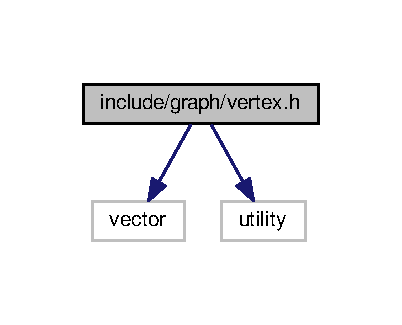
\includegraphics[width=193pt]{vertex_8h__incl}
\end{center}
\end{figure}
This graph shows which files directly or indirectly include this file\+:
\nopagebreak
\begin{figure}[H]
\begin{center}
\leavevmode
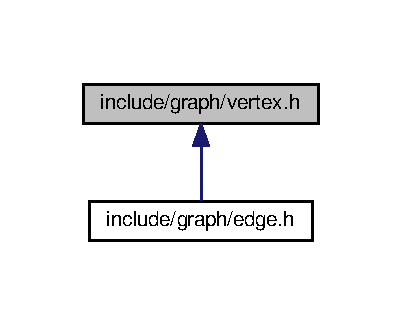
\includegraphics[width=193pt]{vertex_8h__dep__incl}
\end{center}
\end{figure}
\subsection*{Classes}
\begin{DoxyCompactItemize}
\item 
class \hyperlink{classgnm_1_1_vertex}{gnm\+::\+Vertex$<$ T, N $>$}
\begin{DoxyCompactList}\small\item\em \hyperlink{classgnm_1_1_vertex}{Vertex} of a graph with N adjacency lists. \end{DoxyCompactList}\item 
class \hyperlink{classgnm_1_1_vertex_3_01_t_00_011_01_4}{gnm\+::\+Vertex$<$ T, 1 $>$}
\end{DoxyCompactItemize}


\subsection{Detailed Description}
File containing the structure of vertex.

\begin{DoxyAuthor}{Author}
\href{mailto:gnunes.moura@gmail.com}{\tt gnunes.\+moura@gmail.\+com} (Gustavo Nunes) 
\end{DoxyAuthor}

%--- End generated contents ---

% Index
\backmatter
\newpage
\phantomsection
\clearemptydoublepage
\addcontentsline{toc}{chapter}{Index}
\printindex

\end{document}
